\documentclass[12pt]{article} % font size here: some require 11 or 12 point
\usepackage{setspace}
\usepackage{fancyvrb}
\usepackage{epsfig}
\usepackage{fullpage}
\usepackage[small,compact]{titlesec}
\usepackage{times}
\usepackage{enumitem}
\usepackage{wrapfig}
\setlength{\topmargin}{+0.0in}   %%%%%%%%% this is hacked (from +.0.1in) so that it looks right when converted.
\setlength{\oddsidemargin}{-0.0in}
\setlength{\evensidemargin}{-0.0in}
\setlength{\textheight}{9.0in}
\setlength{\textwidth}{6.5in}
\usepackage[margin=1.0in,headheight=0pt,footskip=20pt,headsep=0.2in]{geometry}
\usepackage{natbib}
% ----------------------------------------------------
\usepackage{setspace}
\singlespacing
%\onehalfspacing % may need to switch to single spacing

\usepackage{natbib}
\usepackage{color}
\bibliographystyle{apj}
\newcommand{\apj}{ApJ}
\newcommand{\apss}{Astrophysics and Space Science}
\newcommand{\aj}{AJ}
\newcommand{\apjl}{ApJL}
\newcommand{\mnras}{MNRAS}
\newcommand{\apjs}{ApJS}
\newcommand{\pasp}{PASP}
\newcommand{\araa}{ARA\&A}
\newcommand{\aap}{A\&A}
\newcommand{\aaps}{A\&AS}
\newcommand{\pasj}{PASJ}
\newcommand{\prd}{Phys. Rev. D}
\newcommand{\nat}{Nature}
\newcommand{\nar}{New Astronomy Review}
\newcommand{\ao}{Applied Optics}
\newcommand{\physrep}{Physics Reports}
\newcommand{\etal}{et al}
\def\subsun{\mbox{$_{\odot}$}}
\def\lesssim{\mathrel{\hbox{\rlap{\hbox{%
 \lower4pt\hbox{$\sim$}}}\hbox{$<$}}}}
\def\gtrsim{\mathrel{\hbox{\rlap{\hbox{%
 \lower4pt\hbox{$\sim$}}}\hbox{$>$}}}}
\RequirePackage{natbib}
%\usepackage{setspace}
\setlength{\bibsep}{0.0pt}
\newenvironment{itemize*}%
{\begin{itemize}%
  \setlength{\itemsep}{0pt}%
    \setlength{\parskip}{0pt}}%
{\end{itemize}}

\newenvironment{enumerate*}%
{\begin{enumerate}%
  \setlength{\itemsep}{0pt}%
    \setlength{\parskip}{0pt}}%
{\end{enumerate}}

\usepackage{fancyhdr}
\pagestyle{fancy}

\def\changemargin#1#2{\list{}{\rightmargin#2\leftmargin#1}\item[]}
\let\endchangemargin=\endlist 


\usepackage{fancyhdr}
\pagestyle{fancy}
\lhead{Dwarf Galaxies with Individual Stars}
\rhead{}

%\usepackage[pagestyles]{titlesec}
%\newpagestyle{mystyle}{\sethead{}{}{Name -- Number}\setfoot{}{\thepage}{}}
%\pagestyle{mystyle}

\title{\vspace{-5ex} \Large Galactic Chemical Evolution in the Smallest Galaxies with Individual Stars
       \vspace{-2ex}}
\author{\small PI: Andrew Emerick, Carnegie Observatories and California Institute of Technology, Pasadena, CA \\
\small co-I: Alex Ji, Carnegie Observatories, Pasadena, CA \\
\small co-I: John Wise, Georgia Institute of Technology, Atlanta, GA
}
%\author{Co-I:}
\date{\vspace{-5ex}}
\begin{document} \thispagestyle{empty}

% Star-by-Star Stellar Feedback and Chemical Evolution in Dwarf Galaxies

\maketitle

\begin{changemargin}{0.75cm}{0.75cm} 
\begin{center}\centering \textbf{Summary}\end{center}

We request \textbf{XXX SUs} on the TACC machine Stampede2 utilizing SKX nodes to run the first ever set of cosmological hydrodynamics simulations following the chemical evolution of the first galaxies with individual star particles using the well-tested code \textsc{Enzo}. We request \textbf{7.3 TB} of archival storage on the TACC Ranch system for the data products from this run.
\end{changemargin}

\section{Introduction}
The early formation histories of [ultra-faint?] dwarf galaxies probe some of the most important and extreme regimes of galaxy formation, nucleosynthesis, and cosmology.

Stellar abundances are the key for understanding the early formation histories of dwarf galaxies.

\textbf{In the past decade, observations of stellar abundances in dwarf galaxies have outpaced models for these abundances.}

We currently tend to model mean trends but not the scatter, because scatter is hard and requires simulations.

For the early history of dwarf galaxies, it is now computationally feasible to...

Present-day stellar abundance patterns are tracers of the integrated history of galactic evolution. Ongoing and upcoming observations of detailed stellar abundance patterns, including SEGUE \citep{Yanny2009}, RAVE \citep{Kunder2017}, APOGEE \citep{Anders2014}, APOGEE-2 \citep{Majewski2016}, GALAH \citep{Buder2018}, and the Pristine survey \citep{Starkenburg2017} have obtained an unprecedented number of stars with detailed, multi-element abundances in both the Milky Way and dwarf galaxies in the Local Group. This is in addition to the ongoing work obtaining detailed abundances of $\sim$100 or more stars by multiple groups \cite[e.g.][ (need more!) ]{Hill2019} in low-mass dwarf galaxies in the Local Group. This allows us to directly probe the information-rich scatter in stellar abundance patterns across a range of environments and at low metallicities where the scatter is a more sensitive tracer of underlying galaxy evolution physics. These abundance patterns are the convolution of a galaxy's accretion and merger history, star formation history, internal dynamic structure, mixing timescales and efficiencies in the interstellar medium (ISM), stellar nucleosynthesis, and the effectiveness of stellar feedback in driving metal-rich galactic outflows. \textbf{last sentence}

The quality of these observations are rapidly outpacing our ability to simulate them, in large part because constructing such a model is complex.  Since most metals are released through stellar winds, supernovae, or other similar energetic events, this model requires a detailed understanding of the role of stellar feedback in driving galactic evolution, a current open question in our field.  In addition, models of galactic chemical evolution often lack an exact description for how metals mix within a multi-phase interstellar medium (ISM) and enrich future populations of stars.

\textbf{motivate need to study high-z galaxy formation and evolution and connection to UFDs and low mass dwarfs}

Since \cite{Tinsley1980}, its been understood that the evolution of stellar abundance ratios as a function of metallicity (or, commonly, [Fe/H]) traces different chemical enrichment timescales. The most common example is the ``knee" feature seen in plots of $[\alpha$/Fe] vs. [Fe/H] which represents the transition from core collapse supernova dominant enrichment (high $[\alpha$/Fe]) to significant contributions of Type Ia SNe (Fe, but no $\alpha$). Similar trends can be expected for elements of different nucleosynthetic channels, such as the s-process in AGB stars, and elements with trends in yields as a function of stellar mass. Each of these probe unique timescales in chemical evolution history. However, extracting information about these timescales from stellar abundances is complicated by the fact that the details of galaxy evolution -- stellar feedback, star formation rate, IMF slope, and efficiencies of metal mixing in the ISM -- drives significant scatter in elemental abundances ratios that makes interpreting any evolution quantitatively nearly impossible.

Doing this requires the type of simulations proposed here whereby the details of galaxy evolution are resolved to high-resolution, including star formation, stellar feedback, turbulent mixing, the formation of a multi-phase ISM, and a multi-element chemical evolution model that follows the abundances from individual stars. \textbf{These types of simulations have not yet been performed}. By following detailed chemical enrichment in the early Universe in our simulations, we will be able to unlock the connection between stellar abundances in Local Group ultrafaint dwarf galaxies and physics of galaxy evolution in the early Universe.

%\textbf{Emphasize need for sims with multi-channel enrichment, including mass-dependent yields from SN and AGB channels}

\subsection{Key Scientific Questions and Goals}

We provide a summary of the key scientific questions addressed by the simulations proposed in this project. These simulations are uniquely suited to address each of these issues, and the use of Stampede-2 is necessary to carry these out:

\begin{itemize}
    \item 
\end{itemize}


\section{Proposed Computational Method and Model}

Our simulations will be carried out using the publicly available cosmological adaptive mesh refinement (AMR) hydrodynamics and N-body code \textsc{Enzo} \citep{Enzo2014,Enzo2019}. \textsc{Enzo} is well-tested and has been used extensively in a variety of applications including studies of the ISM and molecular clouds \citep[e.g.][]{Slyz2005,TaskerBryan2008,Jin2017}, the intergalactic medium \citep[e.g.][]{BryanMachacek2000,FangBryan2001,Tonnesen2017}, the first stars and galaxies \citep[e.g.][]{Wise2012a,Oshea2015,Regan2019}, and the roles of stellar feedback in galactic evolution \citep[e.g][]{SalemBryan2014,Goldbaum2016,Forbes2016,Li2019}. We discuss our proposed simulations and relevant methods below, and include a more detailed description of the grid hierarchy and parallelization strategy (including load balancing) in the scaling document. 

\subsection{Initial Conditions}

We build upon the work in \citep{Wise2012a,WiseAbel2012,Wise2014,Corlies2018}, combined with the new star formation and stellar feedback model from \citep{Emerick2019a} following individual star particles, described below. We will use the same set of cosmological initial conditions used in \citep{Wise2012a} to follow the formation of the first generation of dwarf galaxies. The simulation domain is a 1 Mpc (co-moving) box with a root-grid resolution of 256$^3$ and dark matter mass resolution of 1840~M$_{\odot}$. The simulation will be run with a maximum of 12 levels of additional refinement for a maximum resolution of 1~pc (co-moving) using a super-Lagrangian refinement scheme \citep{OsheaNorma2008} to refine on baryon overdensities of $3\times 2^{-0.2l}$, where $l$ is the refinement level, dark matter overdensities of 3, and resolving the local Jeans length by at least 4 cells. In addition, we ensure that stellar feedback, metal enrichment, and metal mixing is well-resolved by forcing refinement in a 4-zone sphere around each star particle with active stellar feedback to at least a co-moving resolution of 4~pc. The simulation will begin at redshift z = 130 and we plan to run the simulation until a redshift of z = 7 ($\sim$ 750 Myr), capturing the evolution of dark matter halos between 10$^6$ and 10$^9$ M$_{\odot}$ with anticipated stellar masses between 10$^3$ and 10$^6$ M$_{\odot}$.

\subsection{Hydrodynamics and Gravity}

For this work we employ a direct-Eulerian piecewise parabolic method \citep{ColellaWoodward1984, Bryan1995} to solve the equations of hydrodynamics. This is an explicit, higher-order accurate version of Godunov's method for ideal gas hydrodynamics that uses spatially third-order accurate piecewise parabolic monotonic interpolation. Shock capturing is handled with a nonlinear Riemann solver. This base method is extended to multiple dimensions using directional splitting, resulting in a final algorithm that is second-order accurate in space and time; we explicitly conserve mass, linear momentum, and energy \citep{Hawley1984, NormanWinkler1986}. We use a dual energy formalism to track the total energy and thermal energy separately, preventing substantial numerical errors that arise when the thermal energy is very small compared to the total energy. We default to using the two-shock approximate Riemann solver \citep{Toro1997}, with progressive fallback to more diffusive approximate Riemann solvers when higher order methods produce negative densities or energies \citep{LemasterStone2009}. 
%In this situation, we fall back to either the Harten-Lax-van Leer (HLL) \citep{Toro1997} method with contact discontinuities -- a three-wave, four-state solver -- or the basic HLL -- a two-state, three-wave solver. 
The hydrodynamics time step is set by the Courant-Friedrichs-Levy (CFL) condition for stability, scaling linearly with cell size ($\Delta x$) and inversely proportional to the sum of the bulk velocity and sound speed in each cell in a given direction. 
%The multidimensional CFL limited time step is the harmonic average of the limiting CFL time step in each dimension.

Gas self-gravity and the gravitational forces of the massive star particles are computed together to compute the gravitational acceleration on each cell and particle. On the root grid, we use a cloud-in-cell (CIC) method \citep{HockneyEastwood1988} to map particles to a time-centered density field, including the effects of particles across sub-grids and neighboring domains; a similar time-centered density field is computed for the baryons in each grid cell. The gravitational potential is solved for using a fast Fourier transform (FFT) in isolated boundary conditions \citep{James1977}; accelerations are computed with a two-point centered difference scheme using the transformed real-space potential. For accuracy on sub-grids, we employ the seven-point, second-order finite difference approximation to Poisson's equation, solving the given Dirichlet boundary conditions with multigrid relaxation. Unwanted oscillations and errors across grids are reduced using expanded buffer zones around each grid, coupled with an iterative relaxation process between sibling grids. Particle accelerations are computed from the grid potential using linear CIC mapping. \texttt{Enzo} employs the particle-mesh N-body method from \cite{HockneyEastwood1988} to evolve the collisionless star particles with an effective force resolution of approximately 2$\Delta x$.

\subsection{Star Formation}

We outline the details of our physics models here, which includes some updates designed specifically for this project since their first development as described in detail in \cite{Emerick2019a}. Star formation occurs stochastically in cells containing cold, dense gas (10$^3$ cm$^{-3}$, $T < 500 K$)) with a converging flow ($\nabla \cdot v < 0$) following a Schmidt law whereby the star formation rate density is given by $\rho_* = \epsilon_{\rm ff} \frac{\rho_g}{t_{\rm ff}}$, where $\rho_g$ is the gas density, $t_{\rm ff}$ is the local gas free-fall time, and $\epsilon_{\rm ff}$ is the efficiency per free-fall time, which we set to 1. In these cells, we stochastically form stars by computing the probability that 200~M$_{\odot}$ of gas will be turned into stars in a given time step. If this occurs, we random sample the stellar initial mass function, depositing individual star particles until at least 200~M$_{\odot}$ of stars form. 

We follow both Pop III star formation and Pop II star formation, with the former occurring only in cells with $Z < 10^{-4} Z_{\odot}$ and $f_{\rm H_2} > 5\times 10^{-4}$ and the latter in metal enriched cells with $Z > 10^{-4} Z_{\odot}$. We adopt a \cite{Salpeter1955}-like IMF for Pop III star formation  above 100~M$_{\odot}$ with an exponential cutoff below this mass and a minimum and maximum particle mass of 11~M$_{\odot}$ and maximum mass of 300~M$_{\odot}$. Pop II star formation follows a \cite{Kroupa2001} IMF with a minimum and maximum mass of 0.08~M$_{\odot}$ and 100~M$_{\odot}$. Upon formation, the stellar abundances of each particle are written to file adopting the local gas abundances from which the stars form.

To reduce computational expense, we merge all Pop II star particles below 2~M$_{\odot}$ in each star forming cell into a single particle. These stars do not have significant feedback or metal enrichment on the timescale of these simulations ($\sim$ 1~Gyr), but still need to be followed as they are the key tracers of stellar abundances in present-day low mass dwarf galaxies.

\subsection{Stellar Feedback}
\textbf{Need to decide what we're doing with PISN. Include them or no? Interesting in both cases, but not sure what would be best?}

We follow a multi-channel stellar feedback prescription capturing stellar winds from massive stars and AGB stars, core collapse and Type Ia supernova, ionizing radiation, Lyman-Werner radiation, and FUV radiation. For both stellar winds and supernovae, mass and energy are deposited into 3-zone radius spherical regions around each star particle. We assume Pop III stars between 11 -40 M$_{\odot}$ and 140 - 260 M$_{\odot}$ and Pop II stars between 8 - 25 M$_{\odot}$ explode as core collapse supernovae at the end of their lives with 10$^{51}$~erg of thermal energy. Stars above 25~M${\odot}$ outside these ranges are assumed to direct collapse with no energy or mass ejection. Stellar surface temperature, surface gravity, and radius (which help set the radiative properties of stars), and lifetimes are adopted from the PARSEC \citep{Bressan2012,Tang2014} stellar evolution grid.

While stellar winds are potentially an important source of pre-SN feedback \citep{Agertz2013}, their effects are sub-dominant to ionizing radiation. To reduce the computational expense of continually evolving fast ($\sim 10^{3} \rm{km} \rm{s}^{-1}$), hot ($T > 10^{6}$~K) gas for the lifetime of massive stars, we greatly reduce the velocities and energies of our stellar winds to just 10~km~s$^{-1}$ and a thermal energy equivalent to the surface temperature of the star. AGB star winds occur at the end of main sequence for stars below 8~M$_{\odot}$. Their length is determined by the PARSEC stellar evolution tables, and we assume the same fixed velocity of 10~km~s$^{-1}$ as for the winds from more massive stars. 
\subsubsection{Stellar Radiation and Radiative Transfer}

We follow the H and He ionizing radiation for all stars above 8~M$_{\odot}$ using \cite{Schaerer2002} for Pop III stars and the OSTAR2002 \citep{Lanz2003} grid of stellar spectra for Pop II stars. Ionizing radiation is followed using the well-tested adaptive ray tracing radiative transfer method of \citep{WiseAbel2011} where photons packages are evolved as rays mapped to a \textsc{HEALPix} grid, adaptively refined as they radiate from their source. To reduce computational expense -- particularly in optically thin regions -- we use source clustering to allow rays to merge once they have travelled far from their source, and limit photon refinement once they have travelled \textbf{XX} kpc from their source. The latter dramatically reduced computational expense when photons escape their galaxy and travel through an optically thin IGM. FUV and LW radiation are both assumed to be optically thin. FUV radiation leads to photoelectric heating of dust grains in the ISM following \cite{Wolfire2003} and the dust-to-gas ratio scaling in \cite{Remy-Ruyer2014}. LW radiation is important for regulating cooling in metal-poor environments by dissociating the dominant coolant, $H_2$. We account for local self-shielding of LW radiation using the method from \cite{Wolcott-Green2011}. To dramatically reduce the computational expense of computing $1/r^2$ radiation for each star particle on each cell, we take advantage of the source clustering tree to speed up this computation by over an order of magnitude when the source count is larger than about 10.

\subsection{Chemical Evolution}

Since we follow individual star particles we can capture detailed, stochastic chemical evolution in our simulations -- a significant improvement over commonly used IMF-averaged yield sets. We use the NuGrid set of stellar yields \citep{Pignatari2016,Ritter2018} to follow the mass and metallicity dependent stellar wind and core collapse supernova abundances of Pop II stars, including AGB winds. This is supplemented with abundances from Slemer et. al. \textit{in prep.} for the stellar winds of stars above the upper mass limit of the NuGrid set, 25~M$_{\odot}$. For Pop III stars, we adopt the core-collapse SNe metal-free yields from \cite{Nomoto2006} for stars between 13~M$_{\odot}$ and 40~M$_{\odot}$ and the PISN yields of \cite{HegerWoosley2002} for stars between 60~M$_{\odot}$ and 130~M$_{\odot}$. Yields for Pop III stars that explode and release metals at the end of their life that are outside these mass ranges adopt the abundances of the closest grid point, scaled by mass. For Type Ia supernovae, we adopt the yields from \cite{Thielemann1986}.

We plan to follow the metal abundances of 8 elements from each of these sources, C, N, O, Mg, Ca, Fe, Sr, and Ba, in addition to the total metallicity and separate fields tracking the fractional contribution of Pop III stars, Pop II core collapse SN, Type Ia SN, and AGB stars to the total metallicity, and a tracer field to model r-process enrichment (discussed below). This gives us a total of 14 metal tracer fields on top of the 9 non-equillibrium chemistry fields. These elements were chosen carefully to maximize both the ability to resolve distinct nucleosynthetic channels and stellar enrichment timescales and usefulness for comparisons to observations, while minimizing the significant additional memory overhead for each additional field.\footnote{Assuming a typical simulation has $\sim10^8$ zones, each tracer field incurs a \textit{minimum} additional run-time memory requirement of 800~MB  (64-bits $\times$ 10$^8$). This represents the on-disk memory requirements for each field in the output data files. In practice, however, the actual run-time overhead is much larger as this does not include the requirements for ghost zones around each grid and additional space in communication buffers. The minimum memory requirement for all 14+9 species fields is 18.4 GB.} \textbf{AE: Do I need this justification for each element?:} O, Mg, and Ca are all produced in significant amounts in core collapse SN, and show a noticeable evolution with supernova progenitor mass, tracing short-timescale ($10~$Myr) chemical evolution. Fe is produced in both core collapse and Type Ia supernova, and the relative abundances of O, Mg, and Ca to Fe traces the evolution between these two yields sources on timescales of 100~Myr to 1~Gyr.\footnote{Additional Type Ia elemental yields (e.g. Ni and Mn) can readily be post-processed using the Type Ia tracer field.}. N, Sr, and Ba all trace s-process enrichment in low-mass AGB stars on timescales of 100~Myr to 1~Gyr, with N and Ba tracing the most massive (4-8~M$_{\odot}$) AGB stars and Sr the less massive ($<4$~M$_{\odot}$). C also has significant production in low-mass AGB stars, but is also produced in core collapse supernova. The C to Fe ratio is an important tracer of early Pop III enrichment. All of these elements are readily observed in a majority of low to medium stellar spectra, with the exception of O. However, O is the most abundant metal species and is used as an important tracer of gas-phase abundances.

Finally, as the origin of r-process enrichment is still highly debated and that possible sources of enrichment are rare and therefore strongly subject to stochastic variations in our simulation volume, we do not include an explicit channel for r-process enrichment. However, as XX - XX M$_{\odot}$ stars are expected to be possible sources of r-process enrichment, we follow their metal enrichment as a separate tracer field that can be used to post-process individual r-process abundances given models for their yields and scaling their expected frequency per XX - XX M$_{\odot}$ supernovae in the simulation. While this does not directly account for NS-NS r-process enrichment, this will test what -- if any -- r-process features in observed abundance patterns can be explained by CCSNe alone, and what features likely require an additional source of enrichment.

\subsection{Test Simulation}

\begin{figure}
\centering
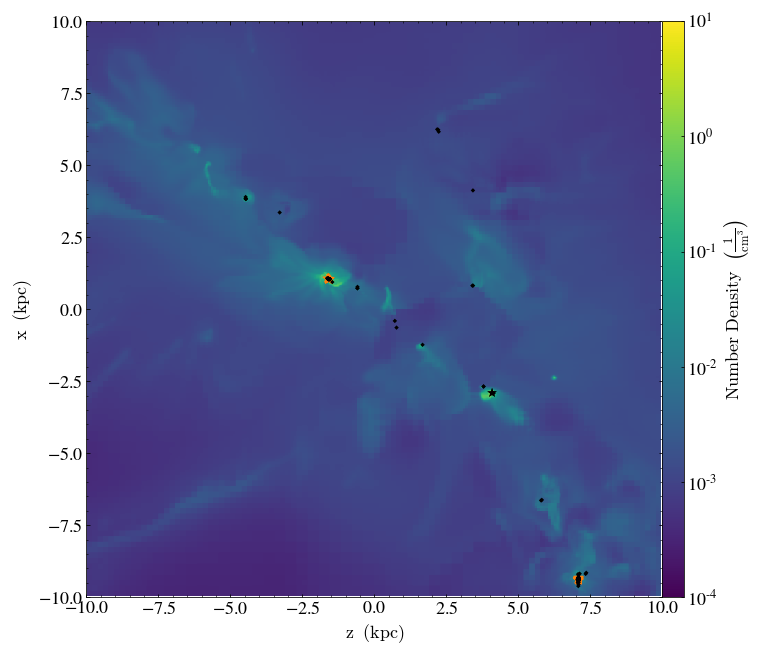
\includegraphics[width=0.45\linewidth]{figures/DD0081_Projection_y_number_density_Metal_Density.png}
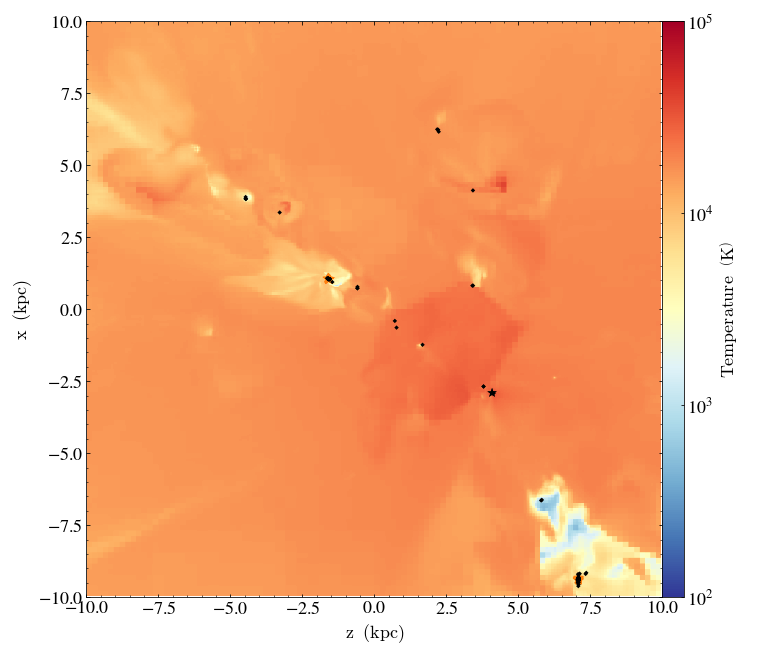
\includegraphics[width=0.45\linewidth]{figures/DD0081_Projection_y_Temperature_Metal_Density.png} \\ 
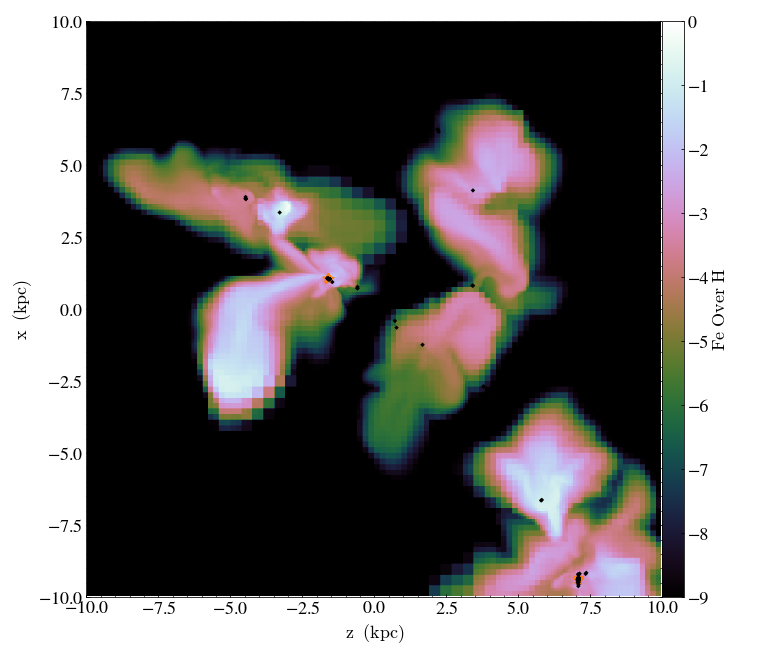
\includegraphics[width=0.45\linewidth]{figures/DD0081_Projection_y_Fe_over_H_Metal_Density.png}
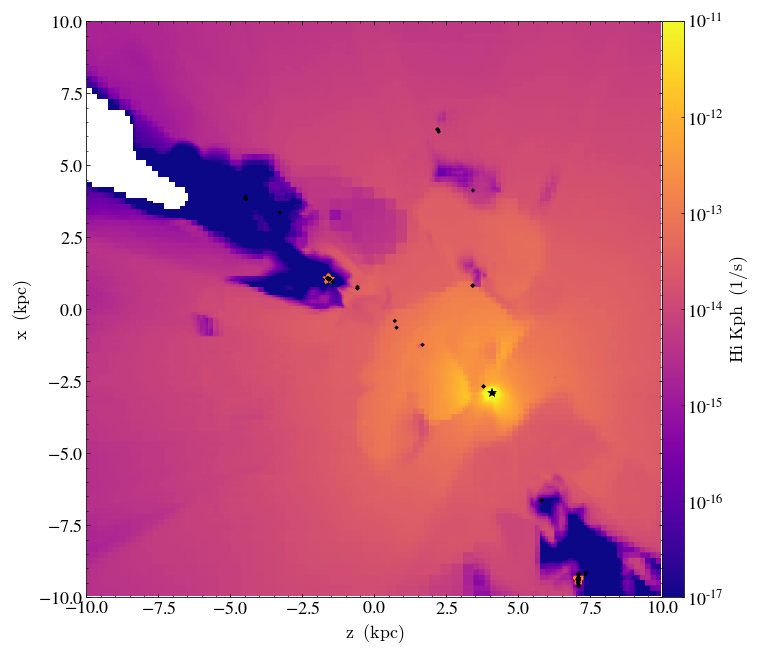
\includegraphics[width=0.45\linewidth]{figures/DD0081_Projection_y_HI_kph_Metal_Density.png}
\caption{\textbf{I'll make this prettier for the final version}. Projections of gas number density, temperature, [Fe/H], and HI ionization rate in a small, low-resolution test simulations using our model of individual star formation and stellar feedback at z = 9.17. Stars are marked as points, with the black diamonds denoting PopIII SN remnants, black stars current main sequence PopIII stars, and orange stars current main sequence Pop II stars.}
\label{fig:test}
\end{figure}

In Figure~\ref{fig:test} we show the results of applying the methods discussed below to a low-resolution (61 co-moving pc, or 6.0~pc at z = 9.0) proof-of-concept test simulation with nested refinement on a single halo. The panels show projections of gas number density, temperature, [Fe/H], and HI ionization rate in the central region of the simulation box. Star particles are marked as black points. By this point in the simulation, a total mass  of $5.0 \times 10^{5}$~M$_{\odot}$ of stars have formed, a majority of which is Pop II star formation, as the Pop III stars that do form ($5.5 \times 10^{3}$~M$_{\odot}$) rapidly enrich this region to above the critial metallicity threshold.
%In addition, in Figure~\ref{fig:test2} we show the gas-phase distributions of


\section{Proposed Computational Resources}

\textbf{The proposed simulation is an incredibly valuable and novel exploration of the questions outlined in the beginning of this proposal.} This will be the first time a simulation of the evolution of the first stars and galaxies using individual star formation and stellar feedback will be performed. For this reason, we propose to devote the resources in our proposal to a single simulation and reserve a wider exploration of the effect of individual feedback processes on this evolution for future work. 

We aim to run our simulations to redshift z $\sim$ 7 as was performed in \cite{Wise2012a}, with regular, frequent data dumps every 5~Myr and 20 targeted redshift outputs at staggered intervals extending from z = 25 to z = 7. These frequent time outputs will be rapidly analyzed to produce significantly smaller data products and images that can be readily stored long-term on local resources for continued analysis. z = 7 corresponds to a simulation time of $\sim$750~Myr, implying a total of 150 + 20 = 170 data outputs. Based on prior experience with the runs in \cite{Wise2012a} and \cite{Emerick2019a}, we anticipate a total cell count of approximately $\sim$10$^{8}$ throughout this simulation (though note that the initial outputs will contain much fewer, with a lower limit of 256$^3$ cells, or $1.68\times10^{7}$). In addition, there will be 256$^3$ dark matter particles. The dark matter particle count will be significantly larger than the star particle count and dominate the particle memory useage, but if we assume a comparable total stellar mass formed as in \cite{Wise2012a} of about $\sim 10^{7}$~M$_{\odot}$ and given the average particle mass in our simulations of 34~M$_{\odot}$ (this is large because we group all stars below 2~M$_{\odot}$ into a single particle per star formation event), we anticipate a total star particle count of about $3 \times 10^{5}$. Our simulation contains 51 total baryon fields and 15 particle fields each stored to high precision as a 64-bit float. This gives us a storage requirement of 64$\times 51 \times 10^8$ + 64$\times 15 \times (1.68\times10^7 + 3\times10^5) = 42.9$~GB per data dump for a \textbf{total storage requirement of 42.9 $\times$ 170 = 7.3~TB.}

The original simulations of \cite{Wise2012a} utilized $\sim$250,000 CPU hours running on 512 cores on a NASA machine. This run -- if used on the Stampede 2 SKX nodes and ignoring processor differences -- translates to 5371 SU (250,000/512 $\times$ 11, where 11 is the number of 48-core nodes needed to have at least 512 total cores) if run on Stampede-2. However, we expect this simulation to be more expensive due to the treatment of stars as individual particles, increasing the star particle count by a factor of $\sim$ 100. This matters most by increasing the number of ionizing sources and the number of distinct particles that are simultaneously interacting with the grid by depositing stellar feedback. The largest increase in cost here is for the ionizing sources. However, the total luminosity should be comparable, and the use of the source clustering algorithm should reduce the raw expense of this increase somewhat.

Based on our test simulations, we achieve \textbf{scaling results and costs here}


\begin{tabular}{c|c|c|c|c|c|c}
\hline
\hline
 Run & Parameter 1 & Parameter 2 & \#cores & \#Nodes & Wall Time (days) & \textbf{SUs} \\
 \hline
     & & & & & & \\
 \hline
 & & & & & Total &
\end{tabular}


\section{Project Team Qualifications}

\textbf{PI Emerick} is a Pasadena Fellow in Theoretical Astrophysics jointly appointed to Carnegie Observatories and the California Institute of Technology in Pasadena, CA. He is a recent PhD recipient from Columbia University advised by collaborator Greg Bryan and collaborator Mordecai-Mark Mac Low. Emerick is a core developer of the \textsc{Enzo}, \textsc{Enzo-E}, and \textsc{Grackle} public-source astrophysical code projects and the primary developer of the star formation, stellar feedback, and chemical evolution routines that will be used in this proposal. He has used \textsc{Enzo} and \textsc{Grackle} in multiple prior publications \citep{Emerick2015,Emerick2018a,Emerick2018b,Emerick2019a,Emerick2019b} and was co-I on a prior successful XSEDE proposal (TG-MCA99S024, "Star Formation, Feedback, and Chemical Evolution of Dwarf Galaxies", PI: Mordecai-Mark Mac Low, 45389.0 SUs on Stampede2) used to conduct the first simulations using the methods outlined in this proposal.

\textbf{co-I JI}

\textbf{co-I Wise}

\section{Management}
\subsection{Summary}

These simulations and any necessary additional code development will be carried out by PI Emerick. The code is currently ready to immediately begin production runs, but we plan to make minor improvements for use ability and efficiency by the allocation start on April 1. co-I Wise developed the initial conditions for these simulations as well as the radiative transfer algorithm, and will advise carrying out and analyzing this work. \textbf{co-I Ji }. In addition, this project will be carried out with collaboration from Greg Bryan (Columbia University / Flatiron Institute) and Mordecai-Mark Mac Low (American Museum of Natural History / Flatiron Institute).

\subsection{Local Computing Environment}

PI Emerick and co-I Ji have access to a computing cluster with 1 PB of total storage and 100 compute nodes each with Intel Xeon E5-2680 v3 (Haswell) processes with 12 cores, 128 Gb of memory. This resource is shared across all of eight of the Carnegie Science institutions and will be valuable for long-term storage of data products from this work and continued analysis, but its shared nature and maximum walltime limit of 2 hours prevents use of this resource for carrying out the proposed simulations. In addition, PI Emerick has access to the ``Wheeler'' $\sim$ 2000 core cluster -- also with Haswell nodes -- at the California Institute of Technology, shared among multiple departments. Its shared nature and small per-user storage ($<$ 2~TB) also prevents using this cluster for more than code development and analysis. \textbf{co-I Wise has...}

\subsection{Other Supercomputing Support}

PI Emerick has access to time on Stampede-2 through allocation TG-AST140064 "Simulating the Milky Way with the LMC" (PI Andrew Wetzel), which is focused on an unrelated project with a different hydrodynamics code, and is PI on startup allocation TG-AST190062 "Chemical Evolution of Ultrafaint Dwarf Galaxies" which was used to perform the scaling tests for this proposal. PI Emerick has recently had access to computing time on NASA Pleiades and Blue Waters, but does not currently have an active allocation with either system and has not applied for computing time for this project on any other resource.
\textbf{co-I Wise...}

------

\pagebreak
\textbf{AE: References will be a separate document and not count towards 10 page limit}
\def\bibfont{\footnotesize}
\bibliographystyle{apj}
\bibliography{msbib}%\thispagestyle{empty}


\end{document}
